\documentclass[compress]{beamer}

\mode<presentation>
{
  \usetheme{Madrid}       % or try default, Darmstadt, Warsaw, ...
  \usecolortheme{default} % or try albatross, beaver, crane, ...
  \usefonttheme[onlymath]{serif}    % or try default, structurebold, ...
  \setbeamertemplate{navigation symbols}{}
  \setbeamertemplate{caption}[numbered]
  \setbeamertemplate{headline}[default]
  \setbeamertemplate{blocks}[rounded][shadow=true]
  \useoutertheme[subsection=false]{miniframes}
} 

\usepackage[utf8]{inputenc}

\usepackage[round]{natbib}
\usepackage{graphicx}
\usepackage{amsmath,amsthm,amssymb}
\usepackage{mathtools}
\usepackage{multicol}
\usepackage[font=footnotesize,textfont=it]{caption}

\AtBeginSection[]{\subsection{}}

\DeclarePairedDelimiter{\abs}{\lvert}{\rvert}
\DeclarePairedDelimiter{\norm}{\lVert}{\rVert}

\let\vec\mathbf
\newcommand*{\C}{%
  \mathbb{C}%
}
\newcommand*{\R}{%
  \mathbb{R}%
}
\newcommand*{\Z}{%
  \mathbb{Z}%
}

\bibliographystyle{IEEEtranN}

\title[Graph Kernels]{Graph Kernels and Support Vector Machines for Pattern Recognition}
\author[Léo Andéol]{\textbf{Léo Andéol}\thanks{leo.andeol@gmail.com}\\ \footnotesize Supervised by: Prof. Hichem Sahbi}
\institute[Sorbonne Uni.]{Master DAC - Sorbonne Université}
\date{May 2019}

\begin{document}

\begin{frame}
  \titlepage
\end{frame}

\section{Motivation and Objectives}
\begin{frame}{Summary}
  \tableofcontents[currentsection]
\end{frame}
\begin{frame}{Motivation and Objectives I}
\begin{multicols}{2}
	\begin{itemize}
		\item Data as graphs : proteins, social networks, ..
		\item Comparing them would be useful : classification, clustering
		\item Big Data : many, large graphs
	\end{itemize}
	\begin{figure}
		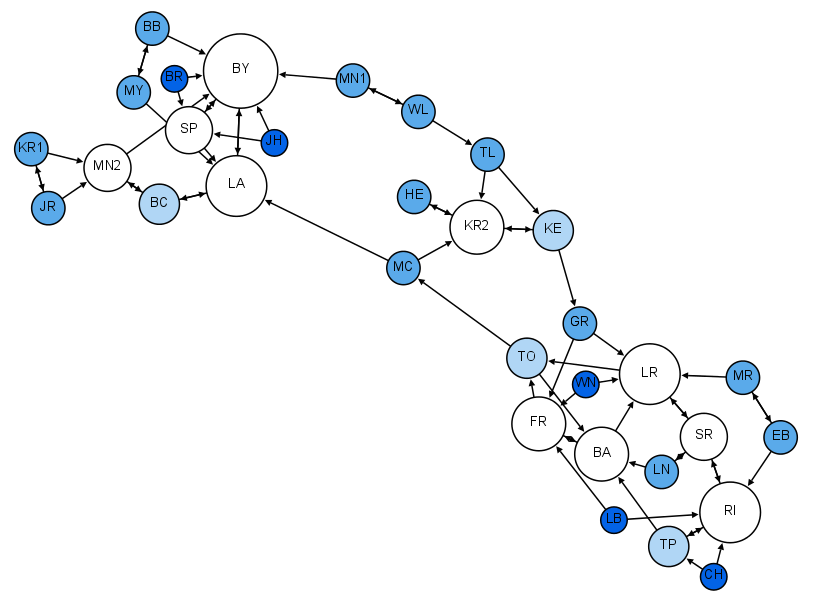
\includegraphics[height=.3\textheight]{data/sociogram.png}\par
		\caption*{\footnotesize Moreno's sociogram (Source : Wikipedia)}
	\end{figure}
\end{multicols}

\begin{figure}
	\centering
	\vspace*{-0.5cm}
	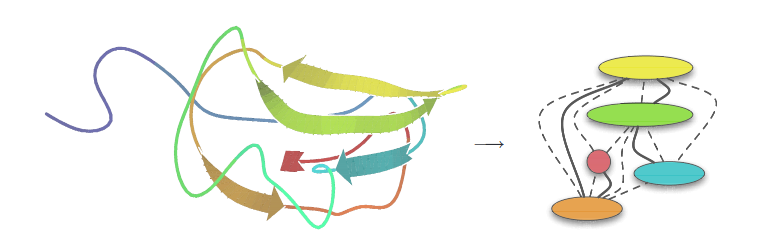
\includegraphics[height=.25\textheight]{data/ecoli.png}
\caption*{Fragment of a protein transformed into a graph \citep{vishwanathan_graph_2010}}
\end{figure}

\end{frame}

\begin{frame}{Motivation and Objectives II : Current methods}
	\begin{block}{Support Vector Machine \citep{cortes_support-vector_1995}}
		\begin{itemize}
			\item Operates on vectorial
			\item Great accuracy
			\item Great capacity of generalization
			\item Allows the use of kernels in its dual form
		\end{itemize}
	\end{block}
	\begin{block}{Kernels}
		\begin{itemize}
			\item Maps data to higher dimensions
			\item Allows functions to replace the dot product
			\item Improves the accuracy of SVMs
		\end{itemize}
	\end{block}
\end{frame}

\begin{frame}{Motivation and Objectives III}
\begin{itemize}
	\item These methods are adapted to \textbf{vectorial data}
	\item Graphs are not
	\item Vectorizing adjacency matrices does not solve the problem (isomorphism)
	\item New types of kernels were discovered
	\item They are very \textbf{complex} to compute
\end{itemize}
\begin{figure}
	\begin{multicols}{2}
		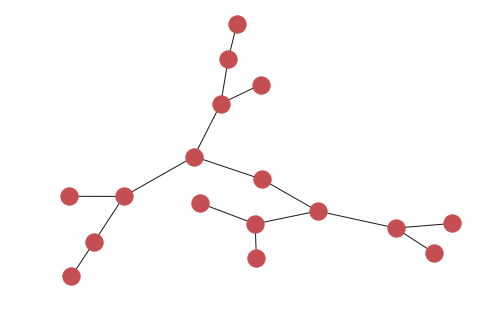
\includegraphics[width=\linewidth]{data/graphs/big_graph_no_label.png}
		\caption*{A tree graph}\par
		$\begin{pmatrix}
		0 & 1 & 0 & 0 & 1 & 0 & 0 & 0 \\ 
		0 & 0 & 0 & 0 & 0 & 0 & 1 & 0 \\
		0 & 0 & 0 & 0 & 0 & 0 & 0 & 0 \\
		0 & 0 & 1 & 0 & 0 & 0 & 1 & 0 \\
		0 & 0 & 0 & 0 & 0 & 0 & 0 & 0 \\
		1 & 1 & 1 & 0 & 0 & 0 & 0 & 0 \\
		0 & 0 & 0 & 0 & 0 & 0 & 0 & 0 \\
		0 & 0 & 0 & 0 & 0 & 0 & 1 & 0 \\
		\end{pmatrix}$
		\caption*{An adjacency matrix}
	\end{multicols}
\end{figure}
\end{frame}


\section{Methodology}
\begin{frame}{Summary}
  \tableofcontents[currentsection]
\end{frame}
\begin{frame}{Support Vector Machines}
\begin{multicols}{2}
	{\begin{itemize}
		\item We have a set of pairs $\{(\vec{x_i},y_i)\}$ of size $N$ where $y_i \in \{-1,+1\}$
		\item We want to maximize the margin, and to minimize the generalization error
		\item We thus minimize
	\end{itemize}
	\begin{equation*}
		\begin{matrix}
		\min_\vec{w} & \frac{1}{2}\norm{\vec{w}}^{2} \visible<2>{+ C\sum\limits_{i=1}^{N}\xi_i}\\
		\textup{s.t.} & y_{i}(\vec{x_i} \cdot \vec{w} + w_{0}) \geq 1\visible<2>{-\xi_i}\\
		1 \leq i \leq N & \visible<2>{\xi_i \geq 0} 
		\end{matrix}
	\end{equation*}}
	\begin{figure}
		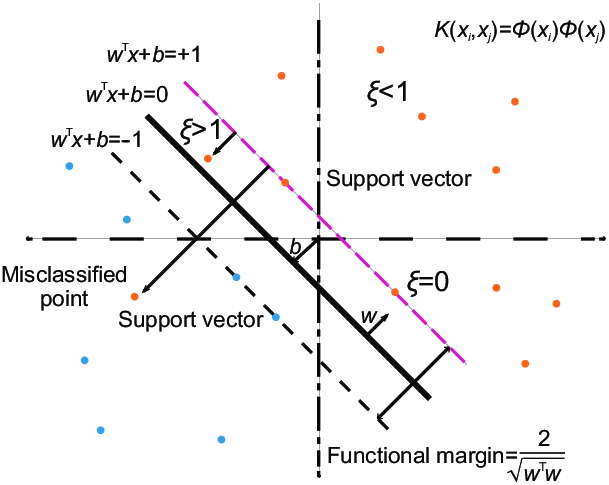
\includegraphics[width=\linewidth]{data/softmargin.png}
		\caption*{Soft-margin SVM \citep{softmargin}}
	\end{figure}
\end{multicols}
\end{frame}
\begin{frame}{Kernels}
	\begin{itemize}
		\item Dual version of the SVM
		\begin{equation*}
		\text{max}_{\vec{w}} \sum\limits_{i=1}^{n} \alpha_i - \frac{1}{2} \sum\limits_{j=1}^{n}\sum\limits_{i=1}^{n}\alpha_{i}\alpha_{j}y_{i}y_{j}\vec{x_{i}}^{\top}\vec{x_{j}}
		\end{equation*}
		\item A map $\phi$ can be used
		\begin{figure}
			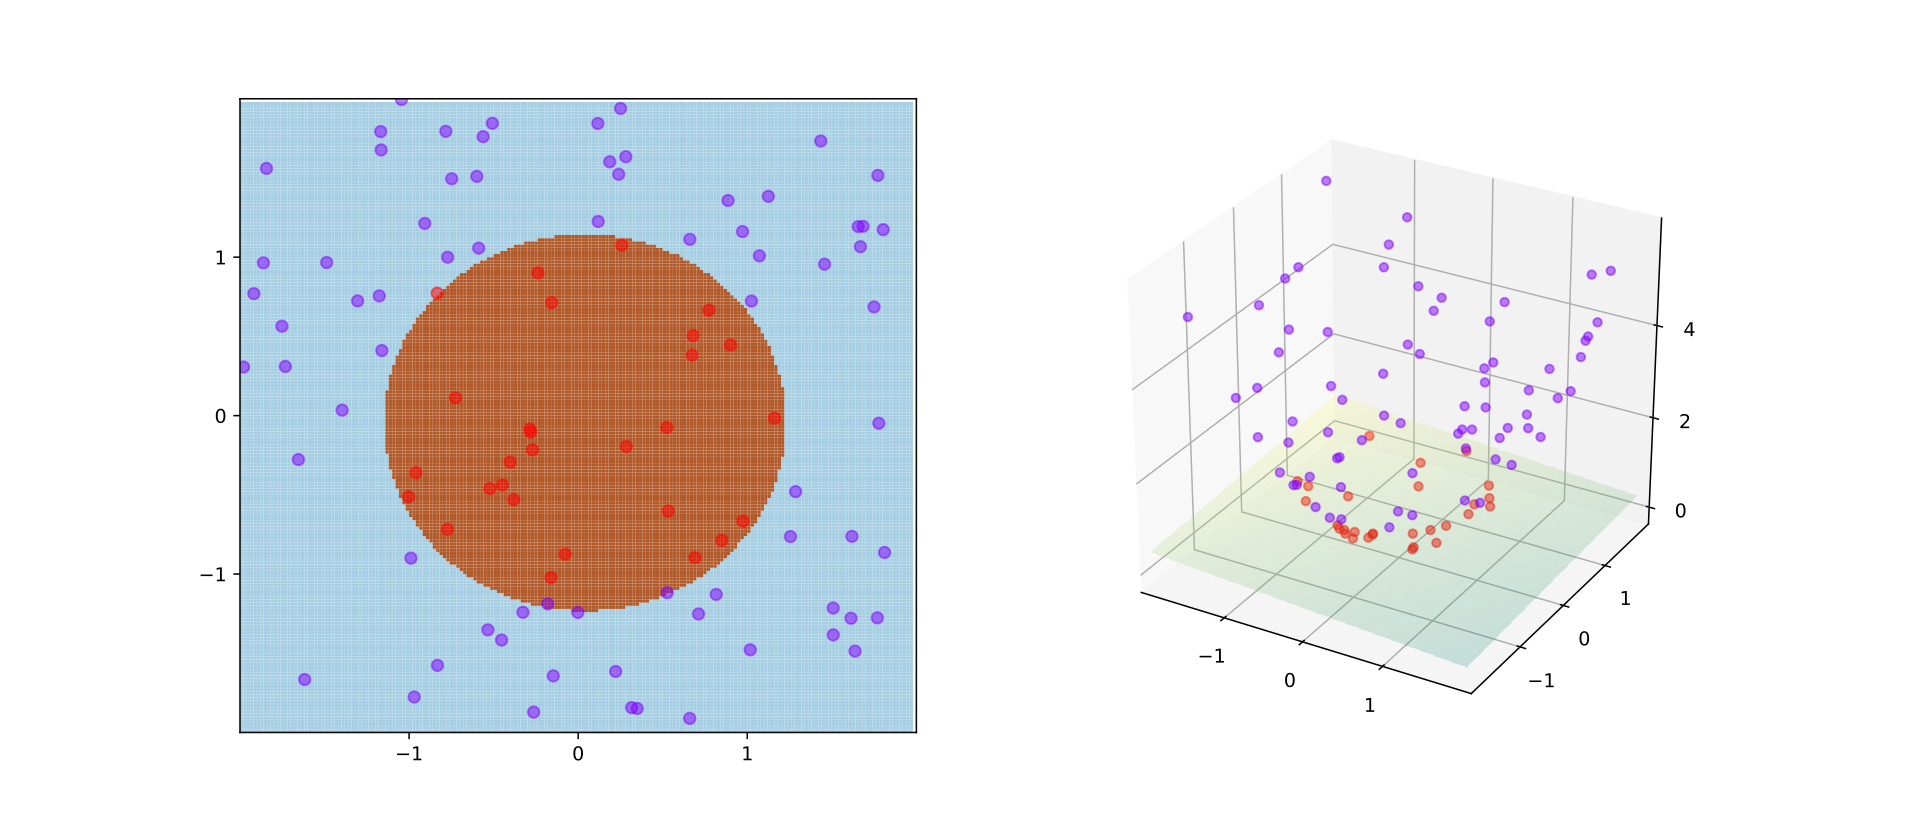
\includegraphics[width=0.7\linewidth]{data/kernel.png}
			\caption{Kernel Trick (Source : Wikipedia)}
		\end{figure}
		\item The dot product can be replaced by a p.s.d function
	\end{itemize}
\end{frame}
\begin{frame}{Graph Kernels}
	\RLmulticolcolumns
	\begin{multicols}{2}
		\vspace*{\fill}
		\begin{figure}
			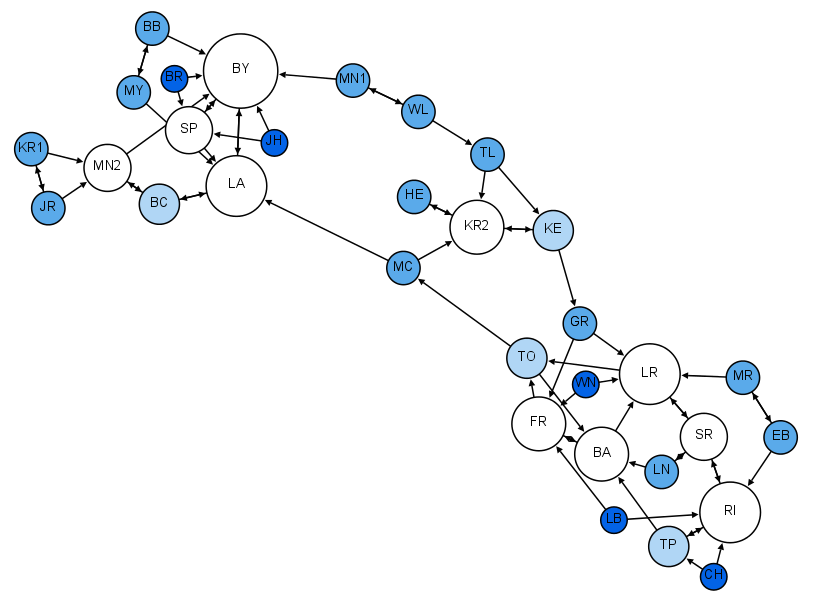
\includegraphics[width=0.7\linewidth]{data/sociogram.png}
			\caption*{\footnotesize Moreno's sociogram (Source : Wikipedia)}
		\end{figure}
		\vfill\null
		\columnbreak
		{We want to classify non \textbf{vectorial data}. There are two types of methods available :
			\begin{itemize}
				\item Kernels on graphs
				\item Kernels on graph nodes
			\end{itemize}
		\pause
		Some graph kernel families :
		\begin{itemize}
			\item Graphlets \citep{shervashidze_efficient_2009}
			\pause
			\item Shortest paths \citep{borgwardt2005shortest}
			\pause
			\item \textbf{Random walks} \citep{vishwanathan_graph_2010}
		\end{itemize}
		$\implies$ The complexity is too large.
		}
	\end{multicols}
\end{frame}
\begin{frame}{Random Walks I}
\begin{multicols}{2}
	Random walks on undirected, connected graphs 
	\begin{itemize}
		\item Starts at a vertex
		\item Randomly picks an edge and moves to the next vertex
		\item Repeats it for a finite (or not) number of steps
	\end{itemize}
	\begin{figure}
		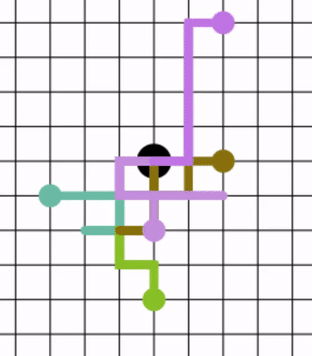
\includegraphics[height=.25\textheight]{data/randomwalk.png}
		\caption*{2D Random walk (Source : Wikipedia)}
	\end{figure}
\end{multicols}
\vspace*{-0.8cm}
\begin{figure}
\begin{multicols}{3}
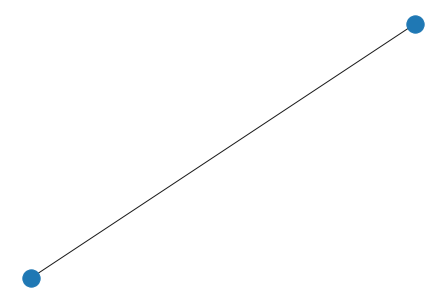
\includegraphics[width=1.5cm]{data/prod_graph/g1.png}\caption*{A graph $G_1$}\par
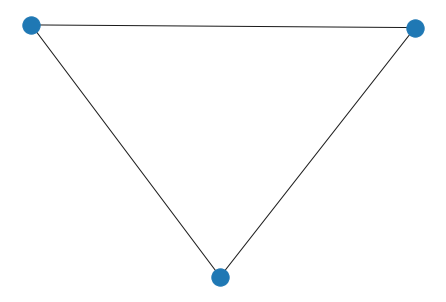
\includegraphics[width=1.5cm]{data/prod_graph/g2.png}\caption*{A graph $G_2$}\par
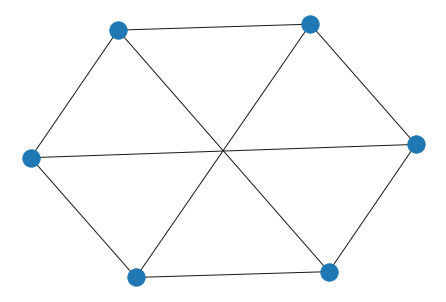
\includegraphics[width=1.5cm]{data/prod_graph/gx.png}\caption*{$G_{\times}=G_1 \otimes G_2$}\par
\end{multicols}
\end{figure}
\begin{itemize}
	\item Computing a random walk on a product graph is equivalent to computing a common walk on both graph \citep{imrich2000product}
	\item The product graph is computed using the Kronecker product $\otimes$
\end{itemize}
\end{frame}
\begin{frame}{Random Walks II}
	\begin{itemize}
		\item Unlabeled product graph : $W_{\times}=A_1\otimes A_2$
		\item Labeled product graph : $W_{\times}=\sum\limits_{l=1}^{d} A_1^{(l)} \otimes A_2^{(l)}$
	\end{itemize}
	\begin{equation*}
	\kappa(G_1,G_2) = \sum\limits_{k=0}^{\infty}\mu(k)q_{\times}^{\top}W_{\times}^{k}p_{\times}
	\end{equation*}
	\begin{itemize}
		\item $p_\times$ and $q_\times$ resp. start and end probabilities : priors $\implies$ uniform probabilities
		\item $\mu(k)$ accentuates walks of certain lengths
	\end{itemize}
\end{frame}
\begin{frame}{Acceleration methods}
\begin{block}{Inverse Kernel}
A special case where $\mu(k)=\lambda^k$ leads to the following kernel
	\begin{equation*}
	\kappa(G_1,G_2)=q_{\times}^{\top}(I-\lambda W_\times)^{-1}p_{\times}
	\end{equation*}
\end{block}
\begin{itemize}
	\item $O(n^6)$ complexity
	\item Some methods will try to accelerate it
\end{itemize}
\end{frame}
\begin{frame}{Sylvester Equation}
\begin{itemize}
	\item Currently applicable only to unlabeled graphs
	\item Restricted to $\mu(k)=\lambda^k\quad\implies$ inverse kernel
\end{itemize}
\begin{block}{Method}
	The Sylvester equation we solve is the following
	\begin{equation*}
	A_iXA_j+C=X
	\end{equation*}
	by multiplying $X$ to $q_\times$ we get 
	\begin{equation*}
		q_{\times}^{\top}\text{vec}(X)=q_{\times}^{\top}(I-\lambda W_{\times})^{-1}p_{\times}
	\end{equation*}
\end{block}
\begin{itemize}
	\item The complexity is $O(n^3)$
\end{itemize}
\end{frame}
\begin{frame}{Conjugate Gradient}
	\begin{itemize}
		\item Applicable to unlabeled and labeled graphs
		\item Restricted to $\mu(k)=\lambda^k\quad\implies$ inverse kernel
		\item The matrix should be symmetrized.
	\end{itemize}
	\begin{block}{Method}
		\begin{itemize}
			\item Computes $A=(I-\lambda W_\times)$ and symmetrizes it
			\item Optimizes $Ax=p_\times$
		\end{itemize}
	\end{block}
\begin{itemize}
	\item The complexity is $O(rdn^3)$ for $r$ iterations and $d$ labels
	\item Efficient if the matrix has a small effective rank $r$
\end{itemize}
\end{frame}
\begin{frame}{Fixed Point Iterations}
\begin{itemize}
	\item Applicable to labeled and unlabeled graphs
	\item Restricted to $\mu(k)=\lambda^k\quad\implies$ inverse kernel
\end{itemize}
\begin{block}{Method}
The algorithm iterates on the following function
\begin{equation*}
x_{t+1} = p_\times + \lambda W_{\times}x_t
\end{equation*}
Either until $\norm{x_{t+1}-x_t}<\epsilon$ or a maximum number of iterations is reached.
\end{block}
\begin{itemize}
	\item The complexity is $O(kdn^3)$ for k iterations and d labels
	\item Convergence requires $\lambda \leq \frac{1}{\xi_1}$
\end{itemize}
\end{frame}
\begin{frame}{Spectral Decomposition I}
\begin{itemize}
	\item Currently applicable only to unlabeled graphs
	\item No restrictions on $\mu(k)$
\end{itemize}
\begin{block}{Method}
	\begin{itemize}
		\item Eigendecomposition of the adjacency matrix
		\item Inverse becomes trivial to compute on diagonal matrix
	\end{itemize}
	\begin{equation*}
	\begin{split}
	\kappa(G_1,G_2)=&\sum\limits_{k=0}^{\infty}\mu(k)q_{\times}^{\top}(V_{\times}D_{\times}V_{\times}^{-1})^{k}p_{\times}\\\visible<2-3>{=& q_{\times}^{\top}V_{\times}\left(\sum\limits_{k=0}^{\infty}\mu(k)D_{\times}^{k}\right)V_{\times}^{-1}p_{\times}}\\\visible<3>{=&
	(q_{1}^{\top}V_{1}\otimes q_{2}^{\top}V_{2})(\sum\limits_{k=0}^{\infty}\mu(k)(D_{1}\otimes D_{2})^k)(V_{1}^{-1}p_{1}^{\top}\otimes V_{2}^{-1}p_{2}^{\top})}
	\end{split}
	\end{equation*}
\end{block}
\end{frame}
\begin{frame}{Spectral Decomposition II}
\begin{itemize}
	\item The complexity is $O(pn^3)$ with $p$ which depends on the complexity of $\mu(k)$
	\item It is even lower since the eigendecomposition of each graph is computed only once
	\item Currently our most efficient method on unlabeled graphs
\end{itemize}
\end{frame}
\begin{frame}{Nearest Kronecker Product Approximation}
\begin{itemize}
	\item Labeled-graph kernel computation can be turned into an unlabeled one with some loss in accuracy, but gain in computation time
	\item The idea is to approximate two matrices $S$ and $T$ such that $\norm{W_\times - A\otimes B}_F$ is minimized
	\item Computed in $O(dn^2)$ time 
	\item All methods such as Spectral Decomposition can then be applied
\end{itemize}
\end{frame}


\section{Experiments}
\begin{frame}{Summary}
  \tableofcontents[currentsection]
\end{frame}
\begin{frame}{Databases and metrics}
    \begin{block}{Synthetic Database}
    	A database of toy data was required to verify claims made in the studied article. A generator was written that can make graphs of "star", "tree" and "ring" types, of different sizes with different labels.
    \end{block}
	\pause
	\begin{block}{Real Databases}
		\begin{itemize}
			\item Proteins : 1113 proteins, 2 classes
			\item Enzymes : 600 enzymes, 6 classes
		\end{itemize}
	\end{block}
	\pause
	\begin{block}{Metrics}
		\begin{equation*}
		L(X,\vec{y})=\frac{1}{\abs{X}}\sum\limits_{i=1}^{\abs{X}}\left\{
		\begin{matrix}
		1 & \mbox{if } f(\vec{x}_i) \neq y_i \\
		0 & \mbox{otherwise}
		\end{matrix}
		\right.
		\end{equation*}
	\end{block}
\end{frame}
\begin{frame}{Implementation}
	%\setlength{\columnsep}{-2.1in}
	\begin{multicols}{2}
		\begin{itemize}
			\setlength\itemsep{4em}
			\item Sylvester Equation\\$A_{1}XA_{2}+C=X$
			\pause
			\item Conjugate Gradient\\$(I-\lambda W_{\times})x=p_{\times}$
			\pause
			\setlength\itemsep{4em}
			\item Fixed point\\$x_{t+1}=\lambda W_{\times}x_{t}+p_{\times}$
			\pause
			\item Spectral Decomposition\\$q_{\times}^{\top}P_{\times}(I-\lambda D_{\times})^{-1}P_{\times}^{-1}p_{\times}$
		\end{itemize}
	\end{multicols}
\end{frame}
\begin{frame}{Performance : Gram matrices}
\begin{table}[!htb]
	\begin{center}
		\begin{tabular}{|p{7mm}|p{9mm}|p{15mm}|p{15mm}|p{15mm}|p{15mm}|p{15mm}|p{15mm}|}
			\hline
			& Raw\newline kernel & Inverse\newline Kernel & Sylvester\newline Equation & Conjugate\newline Gradients & Fixed\newline points & Spectral\newline Decomp. \\
			\hline
			Raw. & 0 & 1.1e-4 & 9.8e-5 & 8.9e-5 & 1.0e-4 & 1.0e-04  \\
			\hline
			Inv. & - & 0 & 2.1e-5 & 7.9e-5 & 4.0e-6 & 6.8e-6 \\
			\hline
			Syl. & - & - & 0 & 8.0e-5 & 1.7e-5 & 1.4e-5  \\
			\hline
			Con. & - & - & - & 0 & 7.9e-5 & 7.9e-5  \\
			\hline
			Fix. & - & - & - & - & 0 & 2.8e-6 \\
			\hline
			Spe. & - & - & - & - & - & 0 \\
			\hline
		\end{tabular}
	\end{center}
	\caption*{MSE of matrix entries}
	\label{tab:frobenius_norm_diff} 
\end{table}
\end{frame}
\begin{frame}{Performance : Gram matrices}
\begin{figure}[!htb]
	\begin{multicols}{3}
		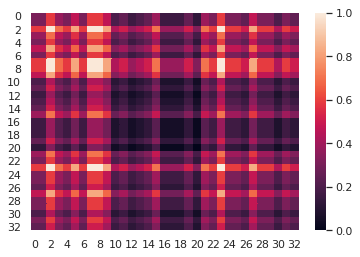
\includegraphics[width=\linewidth]{data/gram/gram3.png}\par
		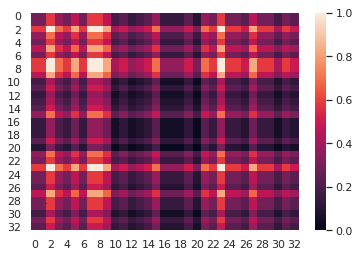
\includegraphics[width=\linewidth]{data/gram/gram4.png}\par
		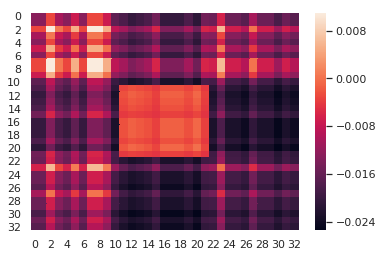
\includegraphics[width=\linewidth]{data/gram/gram5.png}\par
	\end{multicols}
	\caption{A gram matrix computed with the raw method, another with the fixed point method, and the difference between the two}
\end{figure}
\end{frame}
\begin{frame}{Performance : Complexity I}
\begin{figure}[!htb]
	\begin{multicols}{2}
		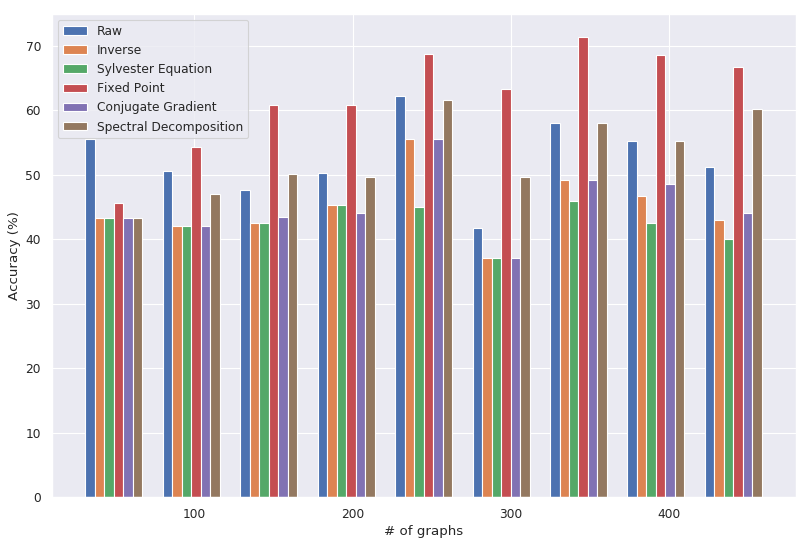
\includegraphics[width=\linewidth]{data/nb_graph/acc.png}\par
		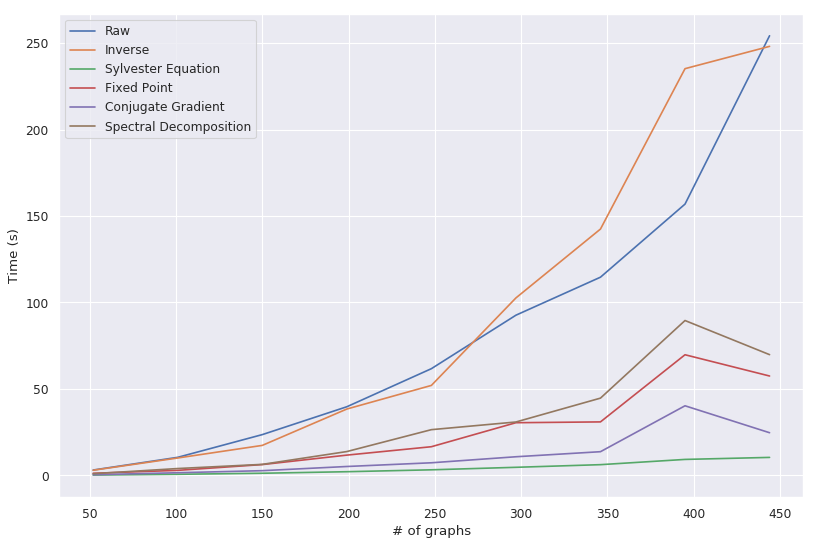
\includegraphics[width=\linewidth]{data/nb_graph/time.png}\par
	\end{multicols}
	\caption {Accuracy and Computation time of different methods depending on the number of graphs}
\end{figure}
\end{frame}

\begin{frame}{Performance : Complexity II}
\begin{figure}[!htb]
	\begin{multicols}{2}
		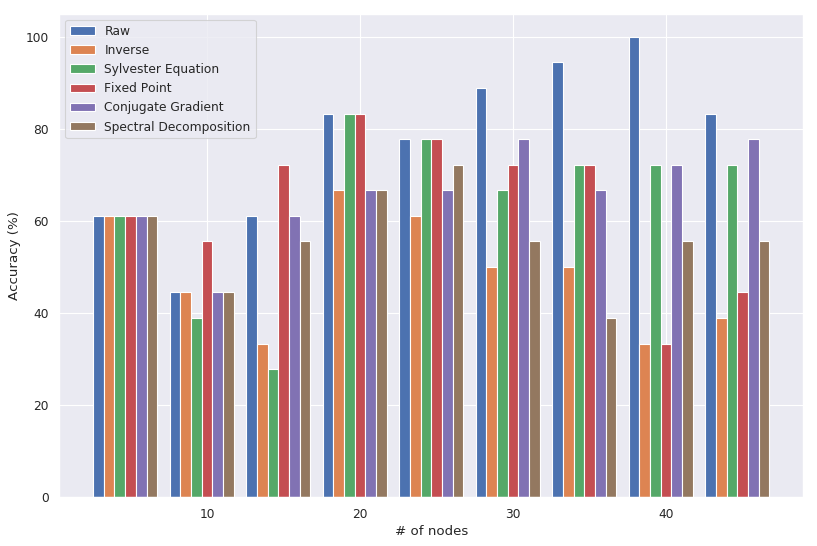
\includegraphics[width=\linewidth]{data/nb_nodes/acc.png}\par
		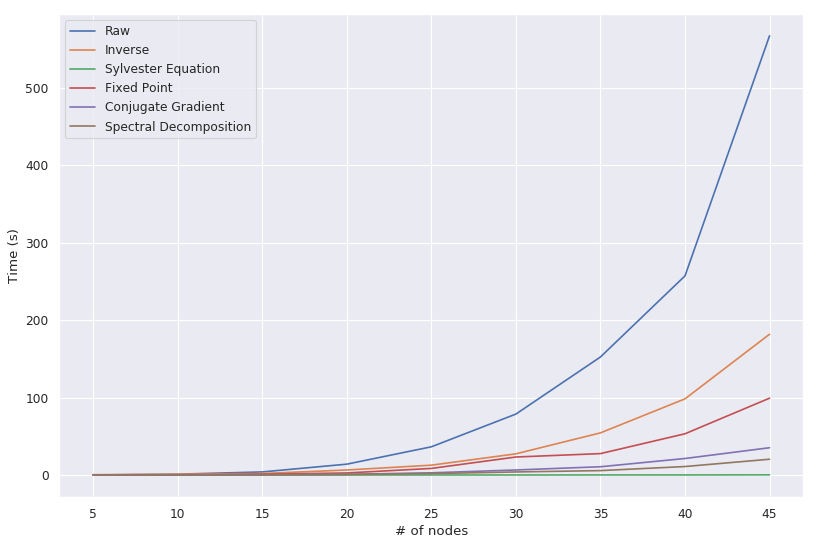
\includegraphics[width=\linewidth]{data/nb_nodes/time.png}\par
	\end{multicols}
	\caption{Accuracy and Computation time of different methods depending on the size of graphs}
\end{figure}
\end{frame}
\begin{frame}{Protein and Enzymes}

\end{frame}


\section{Conclusion}
\begin{frame}{Conclusion}
\begin{block}{Conclusion}
	\begin{itemize}
		\item Random walks : decent accuracy
		\item Several acceleration methods were introduced
		\item Performances are greatly improved
		\item conclusion on real data : todo
	\end{itemize}
\end{block}
\begin{block}{Future work}
	\begin{itemize}
		\item Generalized Sylvester Equation : algorithm and complexity
		\item Generalizing the Spectral Decomposition to labeled graphs
	\end{itemize}
\end{block}
\end{frame}

\renewcommand\bibsection{\subsection{\refname}}
\begin{frame}{References}
\nocite{bondy1976graph,borgwardt_protein_2005,imrich2000product,burges_tutorial_1998,vapnik_statistical_1998,nesterov_lectures_2018,shervashidze_efficient_2009}
\footnotesize
\bibliography{references}
\end{frame}

\appendix
\section[]{Appendix}
\begin{frame}[noframenumbering]{Appendix : Graphs}
\begin{definition}
	A graph\cite{bondy1976graph} is a type of mathematical structure that represents connections between objects. It is more precisely an ordered pair $G=(V,E)$ of two sets: vertices $V$ (or nodes) and edges $E$ that connect two vertices together.
	\begin{equation*}
	E \subseteq \{(u,v) : (u,v) \in V^2\}
	\end{equation*}
\end{definition}
\begin{block}{Properties}
	\begin{multicols}{2}
		\begin{itemize}
			\item Undirected
			\item Labeled or not
			\item Degree
			\item Path and Cycle
		\end{itemize}
		\begin{itemize}
			\item Connected
			\item Tree
			\item Subgraph
			\item Line Graph
		\end{itemize}
	\end{multicols}
\end{block}
\end{frame}
\begin{frame}[noframenumbering]{Appendix : Graphlets}
\begin{figure}
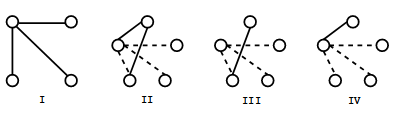
\includegraphics[width=\linewidth]{data/graphlets.png}
\caption*{Some graphlets of size 4 and 5 \citep{shervashidze_efficient_2009}}
\end{figure}
\begin{definition}
Let $G$ and $G_2$ be two graphs, $\vec{f}_G$ and $\vec{f}_{G_2}$ the frequency vectors of respectively $G$ and $G_2$, then the kernel $\kappa$ is defined as
\begin{equation*}
\kappa(G,G_{2})=\vec{f}_{G}^{\top}\vec{f}_{G_2}
\end{equation*}
\end{definition}
\begin{itemize}
	\item It is a subgraph isomorphism problem
\item Complexity of computing $\vec{f}_G$ is $O(n^k)$
\item Sampling is required	
\end{itemize}
\end{frame}
\begin{frame}[noframenumbering]{Appendix : P.S.D}
	\begin{definition}
		A kernel $K$ is positive semi definite if and only if\\
		\begin{equation}
		\sum\limits_{i=1}^{n}\sum\limits_{i=1}^{n}\kappa(\vec{x_{i}},\vec{x_{j}})c_{i}c_{j} \geq 0 \qquad \forall i \in \{1..n\} \quad c_i \in \R
		\end{equation}
		It is also p.s.d if its gram matrix have non-negative eigenvalues.
	\end{definition}
\end{frame}
\begin{frame}[noframenumbering]{Appendix : Conjugate Gradient}
\begin{multicols}{2}
	\begin{itemize}
		\item The idea is to make the new gradient orthogonal to the former
		\item Convergence guaranteed in $n$ steps to solve $Ax=b$ where $A \in R^{n \times n}$
	\end{itemize}
	\begin{figure}[!htb]
		\centering
		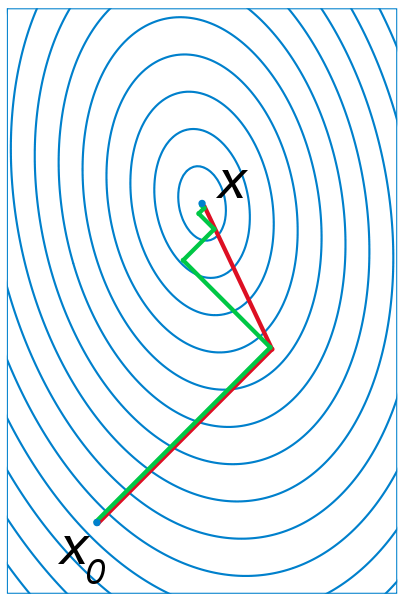
\includegraphics[height=0.5\textheight]{data/sota/conj_grad.png}
		\caption*{Conjugate gradient (red) compared to Gradient Descent (green)}
		\label{fig:conj_grad}
	\end{figure} 
\end{multicols}
\end{frame}
\end{document}